\documentclass[letterpaper,12pt]{article}
\usepackage{mathtools}
\DeclarePairedDelimiter\abs{\lvert}{\rvert}     %serve per mettere il modulo 
\usepackage{booktabs}
\usepackage{bm}
\usepackage{colortbl}
\usepackage{tabularx}
\usepackage{textcomp}
\usepackage{siunitx}
\usepackage{booktabs}
\usepackage{enumitem}
\usepackage{xcolor}
\usepackage{fancyhdr}
\usepackage{caption}
\usepackage{changepage}
\usepackage{amsmath} 
\usepackage{graphicx}
\usepackage{subcaption}
\usepackage[table]{xcolor} 
\usepackage[margin=1in,letterpaper]{geometry} % decreases margins
\usepackage{cite} % takes care of citations
\usepackage[hidelinks]{hyperref} % adds hyper links inside the generated pdf file
% Define the colors
\definecolor{linkcolor}{RGB}{0, 102, 204}
\definecolor{citecolor}{RGB}{34, 139, 34}
\definecolor{urlcolor}{RGB}{255, 69, 0}

% Setup hyperref
\hypersetup{
    colorlinks=false, % colored links
    linkcolor=linkcolor, % color for internal links
    citecolor=citecolor, % color for citations
    urlcolor=urlcolor, % color for URLs
}
\fancypagestyle{logoheader}{
    \fancyhf{}
    \fancyhead[L]{
\includegraphics[width = 3cm]{infn-art-science-universita-degli-studi-di-milano-bicocca-maintainer-universita-studi-milano-bicocca.png}}
    \renewcommand{\headrulewidth}{0pt}
    }
\usepackage{blindtext}
\graphicspath{{immagini/}}
%Required for inserting images
%++++++++++++++++++++++++++++++++++++++++
%Margini 



\begin{document}

\title{{\small Università degli studi Milano-Bicocca  Dipartimento di Fisica - Laboratorio II }\\
    Esperienza Circuiti III}
\author{F. Ballo, S. Franceschina, S. Dolci - Gruppo T1 39}
\date{\today}
\maketitle
\thispagestyle{logoheader}


\begin{abstract}
Nella seguente relazione vengono presentati i risultati ottenuti dalla terza esperienza del corso di Laboratorio II riguardante l'analisi di circuiti elettrici. L'obiettivo di questa esperienza è quello di studiare circuiti RC, RL e RLC in regimi di corrente continua. Imponendo sul circuito, con un generatore di funzioni, un segnale sinusoidale di ampiezza nota, vogliamo ricavare il comportamento del circuito in base alle componenti e in base a dove andiamo a misurare il segnale.
\begin{adjustwidth}{-1cm}{-1cm}
\end{adjustwidth}
\end{abstract}
\tableofcontents
\newpage

\section{Circuiti RC e RL in corrente alternata}

\subsection{Configurazione del circuito e della strumentazione}
Di seguito abbiamo riportato lo schema \ref{fig:config_circuito} utilizzato per riprodurre il circuito in laboratorio con l'utilizzo di una bread-board e degli opportuni componenti. 
\begin{figure}[h!]
    \centering
    \resizebox{0.5\textwidth}{!}{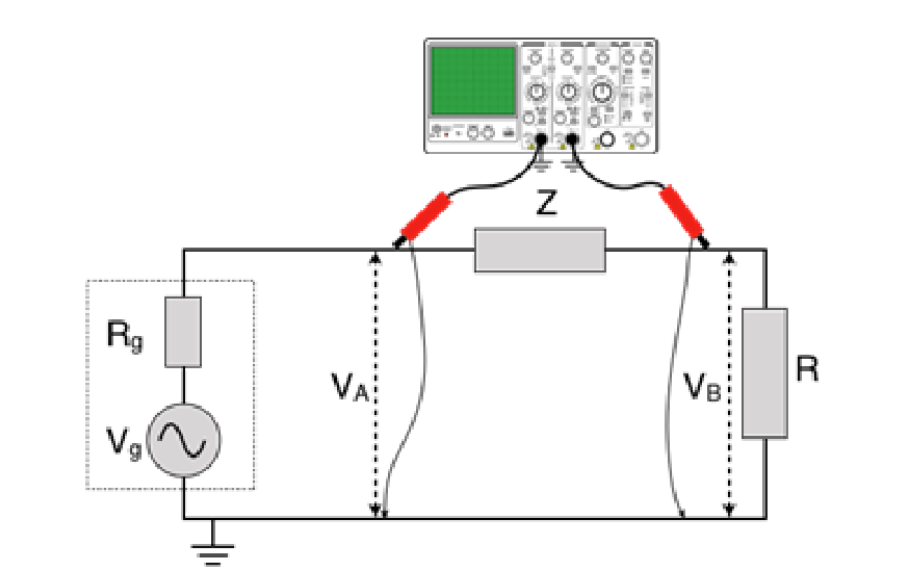
\includegraphics{configurazione circuito.png}}
    \caption{Schema configurazione di circuito, Z rappresenta C o L }
    \label{fig:config_circuito}
\end{figure}
Questa configurazione di circuito rappresenta di fatto un dispositivo lineare a due porte, una di ingresso e uscita. Per studiare il comportamento di circuiti simili ci si rifà alle funzioni di trasferimento, definite come il rapporto tra il segnale in uscita $V_\text{out}$ e segnale in entrata $V_\text{in}$. 
Tali funzioni dipendono dalla frequenza $H = H(\omega)$ del segnale imposta dal generatore; in particolare si tratta di funzioni a variabili complesse: 
$$ H(\omega) = \frac{V_\text{out}(\omega)}{V_\text{in}(\omega)}$$ 
saranno quindi caratterizzate da un modulo e una fase: 
$$ |{H(\omega)| = \frac{|V_\text{out}(\omega)|}{|V_\text{in}(\omega)|}}$$
$$ \phi(\omega) = \phi(\omega)_\text{out} - \phi(\omega)_\text{in} $$
Di seguito riportiamo le funzioni di trasferimento per un circuito RC ai capi della resistenza:
\vspace{3pt}
\begin{equation}
\label{eq:Modulo RC (resistenza)}
    |H_R(\omega)| = \frac{R}{\sqrt{R^2 + \frac{1}{\omega^2C^2}}}
\end{equation}

\begin{equation}
    \label{eq:Fase RC (resistenza)}
    \phi_R = \arctan\left(\frac{1}{R\omega C}\right)
\end{equation}
mentre ai capi del condensatore saranno: 

\begin{equation}
    \label{eq:Modulo RC (condensatore)}
    |H_C(\omega)| = \frac{1}{\sqrt{1 + (R^2\omega^2C^2)}}
\end{equation}

\begin{equation}
    \label{eq:Fase RC (condensatore)}
    \phi_C = \arctan(RC\omega)
\end{equation}

    
\newpage


\subsection{Dati raccolti RC}
Di seguito riportiamo i dati raccolti per la prima parte dell'esperienza. Dopo aver riprodotto il circuito rappresentato nella figura \ref{fig:config_circuito} abbiamo posizionato le sonde dell'oscilloscopio (dopo aver verificato che siano compensate): sonda 1 per misurare $V_\text{in}$ sulla capacità e sonda 2 per misurare $V_\text{out}$ ai capi della resistenza. Le componenti utilizzate per questo circuito sono:

\begin{enumerate}
    \item Resistenza $R = (100.8\pm0.1)\ \Omega$
    \item Capacità $C = (99\pm1$) \text{nF}
\end{enumerate}
Successivamente abbiamo misurato i seguenti parametri al variare della frequenza prodotta dal generatore in un range tra 200 Hz e 3 MHz:
\begin{enumerate}
    \item Ampiezza del segnale $V_\text{in}$
    \item Ampiezza del segnale $V_\text{out}$
    \item Ampiezza della differenza $V_\text{in} - V_\text{out}$
    \item Differenza di fase tra $V_\text{in} - V_\text{out}$ e $V_\text{in}$
    \item Differenza di fase tra $V_\text{in}$ e $V_\text{out}$
\end{enumerate}



\subsection{Analisi dati RC} \label{subsec:Modulo RC}

Come accennato in precedenza, una volta configurato il circuito abbiamo fatto variare la frequenza della tensione in ingresso da 200 Hz a 3 MHz, collezionando misure seguendo un campionamento logaritmico. Per le  misure della tensione ai capi di R e del generatore abbiamo usato un oscilloscopio. Tramite la funzione MATH, abbiamo ricavato la differenza di ampiezza tra i due segnali, trovando così parametri come la tensione ai capi del condensatore. Per la misura delle fasi, abbiamo impostato lo strumento per riportare la differenza di fase tra i segnali in gradi.


\subsubsection{Analisi ai capi della resistenza}
 Per ottenere il modulo della funzione di trasferimento, abbiamo diviso la tensione ai capi della resistenza per la tensione ai capi del generatore; per ottenere il valore della fase abbiamo trasposto le misure dello sfasamento in radianti. \\
Riportiamo di seguito il grafico del modulo della funzione di trasferimento e la curva del fit dei dati seguendo la forma funzionale \ref{eq:Modulo RC (resistenza)} : \\

%Fig
\begin{figure}[h!]
    \centering
    \resizebox{0.7\textwidth}{!}{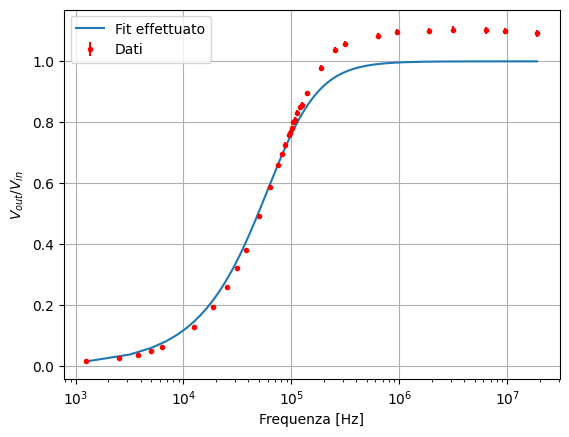
\includegraphics{RC_R_modulo_soprauno.png}}
    \caption{Grafico Modulo - Frequenza sulla resistenza}
    \
    \label{fig:RC_R_modulo_soprauno}
\end{figure}
Analizzando il grafico si può notare un comportamento anomalo: all'aumentare della frequenza il modulo della funzione di trasferimento dovrebbe tendere al valore 1. Al contrario, i nostri dati superano tale valore. Per spiegare questa osservazione abbiamo ipotizzato la presenza di una induttanza parassita, il cui effetto è quello di amplificare la tensione in un intervallo ad alte frequenze. In altre parole, la presenza di un'eventuale induttanza avrebbe aggiunto un picco al grafico una volta sorpassata la frequenza di taglio e poi il grafico sarebbe continuato inalterato. Per verificare l'ipotesi abbiamo raccolto dati ad alte frequenze, estendendo l'intervallo di campionamento, ma ciò è servito a scartare l'ipotesi: la curva resta fermamente al di sopra del valore atteso. \\
Su consiglio degli assistenti di laboratorio abbiamo provato a interpolare con un modello leggermente differente, ipotizzando che il modulo della funzione di trasferimento abbia subito una dilatazione sull'asse delle ordinate. Riportiamo di seguito la forma funzionale modificata e il grafico:
$$\abs{H(\omega)} = k \cdot \frac{R}{\sqrt{R^2+\frac{1}{(\omega C)^2}}}$$ 
\begin{figure}[h!]
    \centering
    \resizebox{0.7\textwidth}{!}{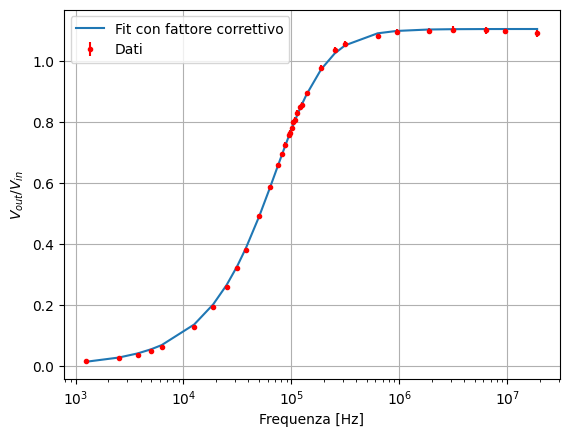
\includegraphics{RC_R_modulo_fattcorrettivo.png}}
    \caption{Grafico modulo-frequenza sulla resistenza con fattore correttivo}
    \label{fig:RC_R_modulo_correzione}
\end{figure}

Abbiamo inoltre estratto dal fit i seguenti parametri:
\begin{enumerate}
    \item Resistenza $R = (100\pm6)\ \Omega$
    \item Capacità $ C = (10\pm 6)\ \text{nF}$
    \item Test Chi-Quadro  $\widetilde{\chi}^2 = 0.8$
    \item p-value$= 0.8 $
    \item Parametro $k = 1.110\pm0.003$
\end{enumerate}
Osserviamo dal grafico che la curva, una volta dilatata in verticale, descrive bene i dati raccolti, sia per basse che per alte frequenze.
\newpage
Per quanto riguarda la fase del segnale sulla resistenza, abbiamo riscontrato lo stesso problema per il calcolo del modulo. Di conseguenza il fit delle misure è stato effettuato di nuovo con un modello correttivo, riportato qui di seguito:

\begin{equation}
    \label{eq:Fase RC (resistenza) correttivo}
    \phi_R = a \cdot \arctan\left(\frac{1}{R\omega C}\right) + b
\end{equation}

\begin{figure}[h!]
    \centering
    \resizebox{0.7\textwidth}{!}{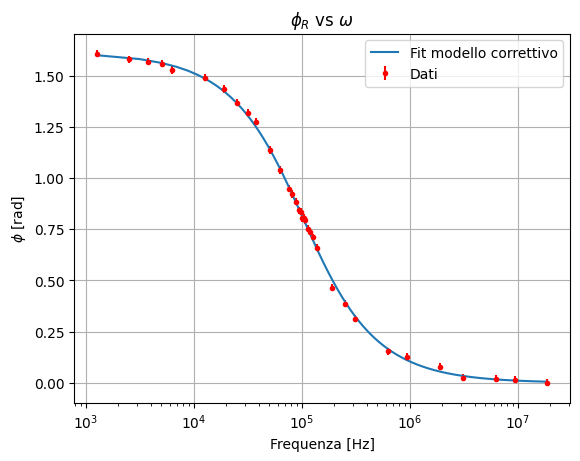
\includegraphics{RC_R_fase_correttivo.png}}
    \caption{Grafico fase-frequenza sulla resistenza con modello correttivo}
    \label{fig:RC_R_fase}
\end{figure}
I dati sembrano seguire meglio questo modello, di seguito riportiamo i parametri estrapolati dal fit:
\begin{enumerate}
    \item Resistenza $R = (99\pm60)\ \Omega$
    \item Capacità $ C = (9.8\pm 6.5)\ \text{nF}$
    \item Test Chi-Quadro  $\widetilde{\chi}^2 = 0.6$
    \item p-value$= 0.95 $
    \item Parametro $ a= 1.03\pm0.01$
    \item Parametro $ b = -4\cdot10^{-4} \pm 7\cdot10^{-3} \approx 0$
\end{enumerate} 
%Per quanto riguarda le incertezze elevate sono dovute al fatto che abbiamo preferito riportare fit con un $\widetilde{\chi}^2$ basso e di conseguenza le incertezze sono salite. Ulteriori considerazioni sulle incertezze elevate sono riportate in seguito(\ref{sec:incertezze}). 
\newpage

\subsubsection{Ai capi del condensatore}
 Di seguito riportiamo i dati per lo studio della funzione di trasferimento ai capi del secondo componente in questo circuito, la capacità.
 Per ottenere il modulo della funzione di trasferimento abbiamo diviso la tensione ai capi della capacità per la tensione ai capi del generatore; per ottenere la fase abbiamo misurato in maniera analoga tramite l'oscilloscopio la differenza di fase fra la tensione in ingresso e la tensione ai capi di C, in seguito abbiamo trasposto le misure in radianti. \\
Riportiamo di seguito il grafico del modulo della funzione di trasferimento e il fit secondo la forma funzionale \ref{eq:Modulo RC (condensatore)}. : \\

%Figure da inserire: grafico modulo funzione di trasferimento e

\begin{figure}[h!]
    \centering
    \resizebox{0.7\textwidth}{!}{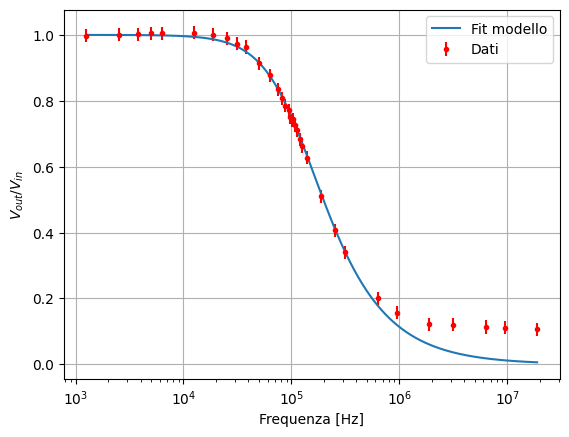
\includegraphics{RC_C_mod_noncorrettivo.png}}
    \caption{Grafico modulo-frequenza sulla capacità}
    \label{fig:RC_C_modulo}
\end{figure}
%tabella con valori di chi quadro, R, C

Analogamente a quanto osservato per la resistenza, osserviamo che il modulo della funzione di trasferimento non tende a zero per frequenze alte, al contrario si attesta ad un valore di poco superiore. Come per la resistenza abbiamo provato a modificare la forma funzionale, dilatandola sull'asse delle ordinate, Riportiamo di seguito la forma funzionale modificata e il grafico:
\newpage
\begin{equation}
    \label{eq:Modulo RC(capacità) correttivo}
    \abs{H(\omega)} = \frac{a}{\sqrt{1+(R\omega C)^2}+b}
\end{equation}


\begin{figure}[h!]
    \centering
    \resizebox{0.7\textwidth}{!}{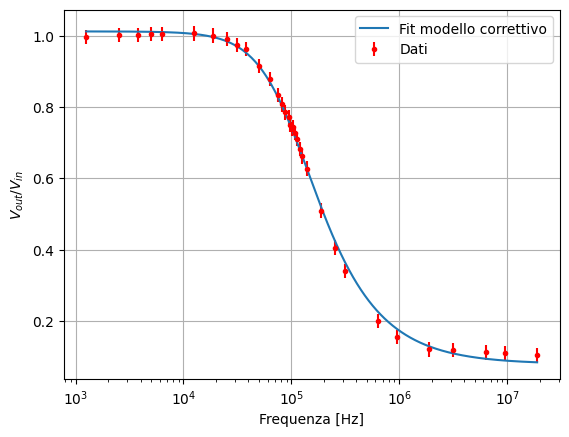
\includegraphics{RC_C_mod_correttivo.png}}
    \caption{Grafico modulo-frequenza sulla capacità, con modello correttivo}
    \label{fig:RC_C_modulo_correzione}
\end{figure}

Si nota dal nuovo grafico che la curva, una volta dilatata in verticale, segue i dati raccolti sia per basse che per alte frequenze.
Abbiamo inoltre estratto dal fit i seguenti parametri:

\begin{enumerate}
    \item Resistenza $R = (100\pm18)\ \Omega$
    \item Capacità $ C = (10\pm2)\ \text{nF}$
    \item Test Chi-Quadro  $\widetilde{\chi}^2 = 0.4 $
    \item p-value$= 0.9 $
    \item parametro $a = 0.93\pm0.01 $
    \item parametro $b = 0.08\pm0.01$
\end{enumerate}

Riportiamo di seguito il grafico delle misure per quanto riguarda la fase della funzione di trasferimento sulla capacità. Come forma funzionale per costruire il seguente grafico abbiamo utilizzato la legge \ref{eq:Fase RC (condensatore)}.

%Figure da inserire: grafico fase funzione di trasferimento e 
\begin{figure}[h!]
    \centering
     \resizebox{0.7\textwidth}{!}{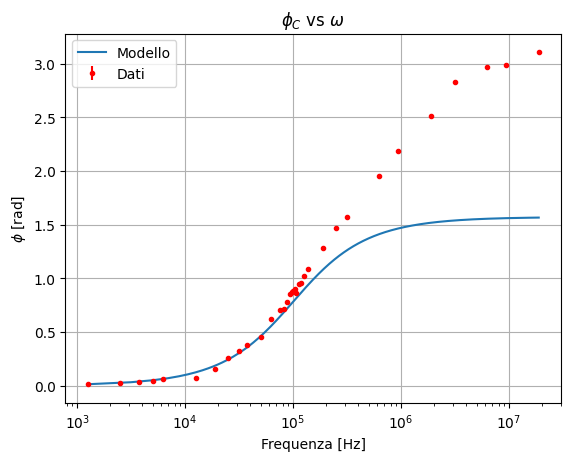
\includegraphics{RC_C_fase.png}}
    \caption{Grafico frequenza-fase sulla capacità  }
    \label{fig:RC_C_fase}
\end{figure}

Come si può notare dal grafico per frequenze basse notiamo che le misure seguono il modello, per poi divergere a frequenze più alte. Purtroppo per mancanza di tempo dovuta a problemi tecnici con la strumentazione non siamo riusciti a riprendere le misure, ad ogni modo supponiamo che la discrepanza provenga dalla presa stessa delle misure. 

\subsection{Conclusioni circuito RC}
Riassumendo quanto ottenuto per il circuito RC, nonostante le misure si discostino dai modelli a meno di correzioni, è stato comunque possibile verificare che effettivamente un circuito RC si comporta come un filtro passo basso, ovvero un circuito RC in serie fa passare frequenze da 0 Hz fino alla frequenza di taglio che nel nostro caso era di circa $10^5 \text{ Hz}$.
%inserire qualche conclusione sui circuiti RC 
%Domande poste dalla scheda sia per RC che RL :  
Riguardo alla precisione delle misure abbiamo notato che nel caso del nostro oscilloscopio, misurare manualmente la fase, tramite differenze tra massimi, ci forniva valori più precisi, tecnicamente una misura tra i passaggi per lo zero sarebbe stata ancora più precisa per via dell'assenza di rumore nel segnale rispetto ai massimi.
Nonostante ciò la forma d'onda Va risultante ai capi dell'impedenza ha mantenuto la stessa forma dell'onda Vg imposta dal generatore, i vari effetti di distorsione ottenuti specialmente a frequenze più alte sono comunque piuttosto comuni e crediamo la ragione principale risieda nella presenza di induttanze parassite negli strumenti di misura che per mancanza di tempo non siamo riusciti a considerare. 
Una domanda posta dalla scheda chiedeva che cosa succederebbe se R e C venissero scambiati,
in generale possiamo dire che ci aspettiamo che il comportamento di filtro passa-basso rimanga inalterato, in generale più che dall'ordine ci aspettiamo che sia la frequenza di taglio a modificare la risposta del circuito e quindi i valori stessi delle componenti.

\subsection{Dati raccolti RL}
Di seguito riportiamo i dati raccolti per il circuito RL. Dopo aver riprodotto lo stesso circuito rappresentato nella figura \ref{fig:config_circuito} cambiando il condensatore con un' induttore abbiamo posizionato le sonde dell'oscilloscopio nel seguente modo: sonda 1 per misurare $V_\text{in}$ induttore e sonda 2 per misurare $V_\text{out}$ ai capi della resistenza.
Le componenti utilizzate per questo circuito sono:
\begin{enumerate}
	\item Resistenza $R = (1040.0 \pm0.1)\ \Omega$
	\item Induttore $L = (0.05\pm 0.01)\ \text{H}$
\end{enumerate}

Successivamente abbiamo misurato gli stessi parametri al variare della frequenza prodotta dal generatore in un range tra 100 Hz e 1 MHz:
\begin{enumerate}
	\item Ampiezza del segnale $V_\text{in}$
	\item Ampiezza del segnale $V_\text{out}$
	\item Ampiezza della differenza $V_\text{in} - V_\text{out}$
	\item Differenza di fase tra $V_\text{in} - V_\text{out}$ e $V_\text{in}$
	\item Differenza di fase tra $V_\text{in}$ e $V_\text{out}$
\end{enumerate}
Le funzioni di trasferimento di un circuito RL sono le seguenti. \\
Ai capi della resistenza:
\begin{equation}
	\label{eq:Modulo RL (resistenza)}
	|H_R(\omega)| = \frac{R}{\sqrt{R^2 + \omega^2L^2}}
\end{equation}

\begin{equation}
	\label{eq:Fase RL (resistenza)}
	\phi_R = \arctan\left(\frac{\omega L}{R}\right)
\end{equation}
E ai capi dell'induttanza:
\begin{equation}
	\label{eq:Modulo RL (induttanza)}
	|H_L(\omega)| = \frac{\omega L}{\sqrt{R^2 + \omega^2L^2}}
\end{equation}

\begin{equation}
	\label{eq:Fase RL (induttanza)}
	\phi_L = \arctan\left(\frac{\omega L}{R}\right)
\end{equation}


\subsection{Analisi dati RL}

\subsubsection{Ai capi della resistenza}

Dopo aver raccolto i dati in modo analogo a quanto fatto per il circuito RC, abbiamo calcolato il modulo e la fase della funzione di trasferimento ai capi della resistenza; i risultati sono stati riportati nei grafici in figura \ref{fig:RL_R_modulo} e \ref{fig:RL_R_fase}. Per quanto riguarda la fase, abbiamo deciso di riportare anche un grafico (figura \ref{fig:RL_R_fase_modello})con i dati sovrapposti alla funzione, avendo però passato come parametri i valori R, L ottenuti dal multimetro palmare; il motivo viene discusso nelle conclusioni.

L'interpolazione dei dati del modulo con la legge (\ref{eq:Modulo RL (resistenza)}) restituisce i seguenti valori per i parametri:
\begin{enumerate} 
    \item $R = (1080 \pm 2000)\ \Omega $
    \item $L = (0.05 \pm 0.1)\ \text{H} $
\end{enumerate}
In seguito abbiamo interpolato i dati della fase seguendo la (\ref{eq:Fase RL (resistenza)}), ricavando i valori che seguono:
\begin{enumerate} %da rivedere
    \item $ R = (1120 \pm 2700)\ \Omega$
    \item $ L = (0.05 \pm 0.1)\ \text{H}$
\end{enumerate}
La concordanza del modello è stata valutata tramite il test del $\chi^2$; di seguito riportiamo i risultati ottenuti.
\begin{enumerate}
    \item Concordanza del modello per il modulo:
$$ \widetilde{\chi}^2 = 2.1, \qquad p-value = 0.0002 $$
    \item Concordanza del modello per la fase:
$$ \widetilde{\chi}^2 = 1.4, \qquad p-value = 0.07$$
\end{enumerate}

\subsubsection{Ai capi dell'induttanza}
Di seguito riportiamo l'analisi dati per le misure effettuate ai capi dell'induttanza
 ottenute sottraendo la tensione ai capi della resistenza con quella del generatore. Abbiamo seguito l'equazione (\ref{eq:Modulo RL (induttanza)}) per il modulo della funzione di trasferimento e la legge(\ref{eq:Fase RL (induttanza)}) per la fase. Ne riportiamo i grafici in figura \ref{fig:RL_L_modulo}, e \ref{fig:RL_L_fase}.\\
Oltre a questi due, abbiamo deciso di riportare in figura \ref{fig:RL_L_modulo_modello} anche un grafico in cui i dati raccolti vengono sovrapposti alla funzione modulo calcolata con i parametri R, L ottenuti tramite misurazione da multimetro palmare; il motivo verrà discusso nelle conclusioni per RL.

Riportiamo i valori ottenuti dal fit del modulo:
\begin{enumerate} 
    \item $R = (1120\pm 1980)\ \Omega $
    \item $L = (0.04 \pm 0.07)\ \text{H}$
\end{enumerate}

Riportiamo anche i valori ottenuti dal fit della fase:

\begin{enumerate} 
    \item $ R = (1040 \pm 2500)\ \Omega $
    \item $ L = (0.05 \pm 0.1)\ \text{H} $
\end{enumerate}

Infine abbiamo ripetuto il test del $\chi^2$ per valutare l'accordo dei dati al modello. \\
\begin{enumerate}
    \item Concordanza del modello per il modulo:
$$ \widetilde{\chi}^2 = 3.6, \quad p-value = 3.9 $$ 
    \item Concordanza del modello per la fase:
$$ \widetilde{\chi}^2 = 1.5, \quad p-value = 0.04 $$ 
\end{enumerate}

Osservando il grafico \ref{fig:RL_L_modulo} si può notare che la curva non tende asintoticamente a 1 ma ad un valore più basso. \\
Per questo motivo, similmente a quanto svolto nella sezione di circuito RC, abbiamo deciso di provare a interpolare i dati tramite un modello correttivo "ad hoc", che tenga conto di una dilatazione e una traslazione in entrambi i casi. In figura \ref{fig:RL_L_modulo_correttivi} è stato riportato il grafico risultante:

Di seguito riportiamo i valori estrapolati dal fit del modulo secondo il modello correttivo:
\begin{enumerate} 
    \item $R = (1100 \pm 2500)\ \Omega$ 
    \item $L = (0.05 \pm 0.1)\ \text{H}$ 
\end{enumerate}
Successivamente abbiamo ripetuto il test del $\chi^2$ per valutare l'accordo dei dati al modello correttivo, ottenendo come valori:

$$ \widetilde{\chi}^2 = 1.5, \quad p-value = 0.04 $$ 

\begin{figure}[p] % First page
    \centering
    \begin{subfigure}[b]{0.45\textwidth}
        \centering
        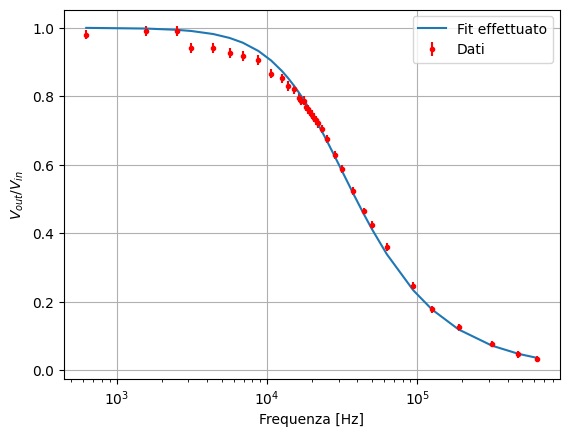
\includegraphics[width=\textwidth]{RL_R_modulo.png}
        \caption{Grafico modulo-frequenza per R, interpolazione}
        \label{fig:RL_R_modulo}
    \end{subfigure}
    \hfill
    \begin{subfigure}[b]{0.45\textwidth}
        \centering
        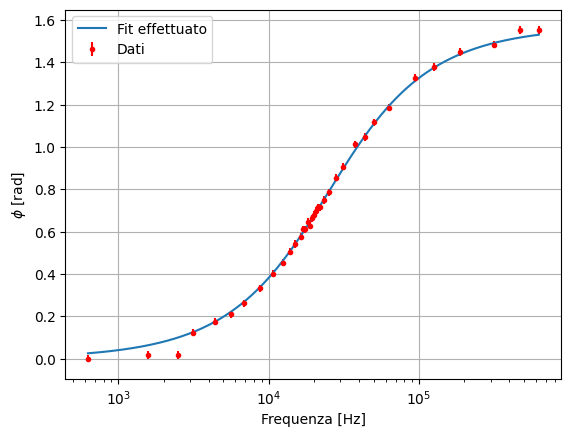
\includegraphics[width=\textwidth]{RL_R_fase.png}
        \caption{Grafico fase-frequenza per R, interpolazione}
        \label{fig:RL_R_fase}
    \end{subfigure}
    
    \begin{subfigure}[b]{0.45\textwidth}
        \centering
        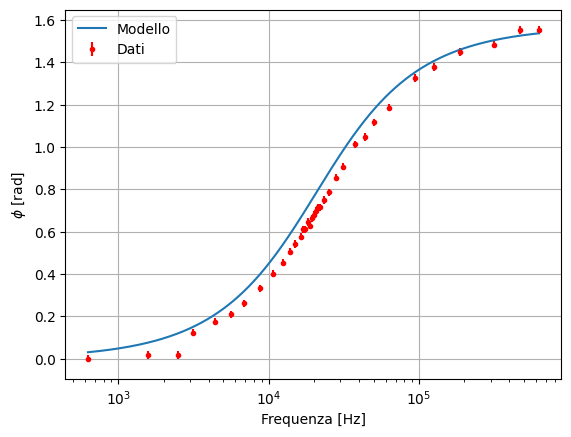
\includegraphics[width=\textwidth]{RL_R_fase_modello.png}
        \caption{Grafico fase-frequenza per R, modello con parametri ottenuti dal multimetro palmare}
        \label{fig:RL_R_fase_modello}
    \end{subfigure}
    \hfill
    \begin{subfigure}[b]{0.45\textwidth}
        \centering
        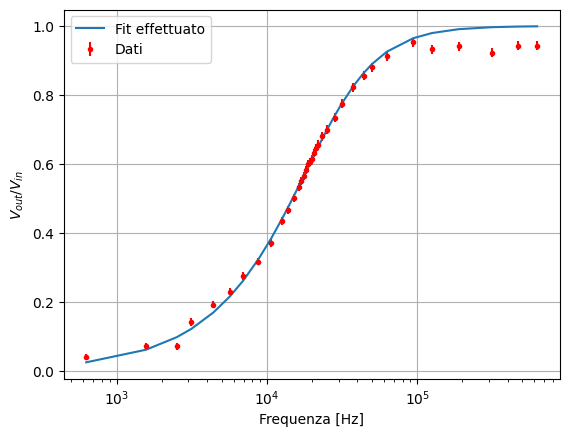
\includegraphics[width=\textwidth]{RL_L_modulo.png}
        \caption{Grafico modulo-frequenza per L, interpolazione}
        \label{fig:RL_L_modulo}
    \end{subfigure}
    \caption{Grafici circuito RL}
    \label{fig:multi1}
\end{figure}

\begin{figure}[p] % Second page
    \centering
    \begin{subfigure}[b]{0.45\textwidth}
        \centering
        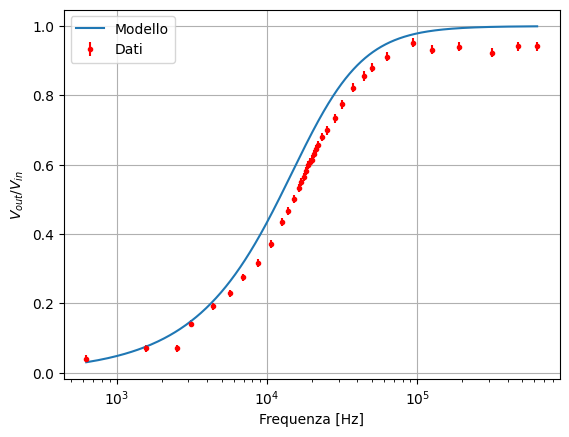
\includegraphics[width=\textwidth]{RL_L_modulo_modello.png}
        \caption{Grafico modulo-frequenza per L, modello con dati presi dal multimetro palmare}
        \label{fig:RL_L_modulo_modello}
    \end{subfigure}
    \hfill
    \begin{subfigure}[b]{0.45\textwidth}
        \centering
        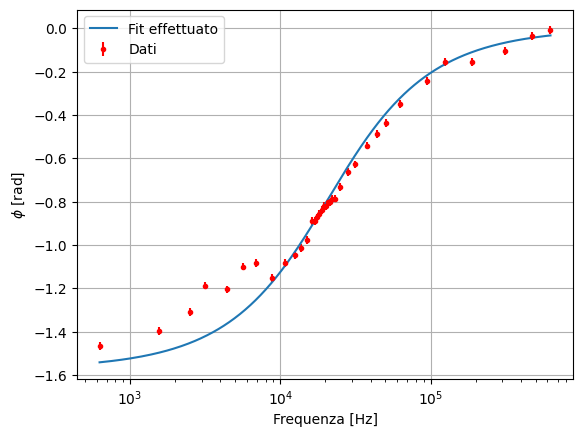
\includegraphics[width=\textwidth]{RL_L_fase.png}
        \caption{Grafico fase-frequenza per L, interpolazione}
        \label{fig:RL_L_fase}
    \end{subfigure}
    
    \begin{subfigure}[b]{0.45\textwidth}
        \centering
        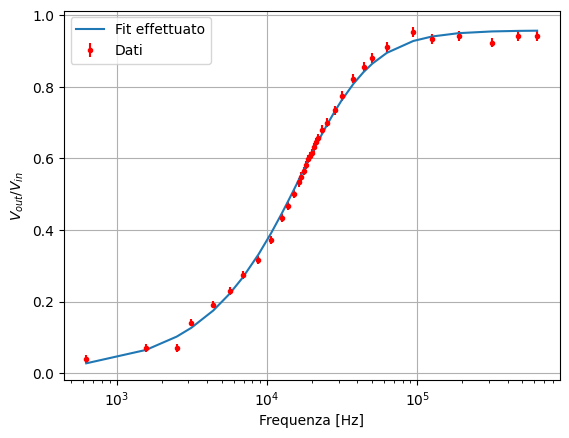
\includegraphics[width=\textwidth]{RL_L_modulo_correttivi.png}
        \caption{Grafico modulo-frequenza per L con modello correttivo}
        \label{fig:RL_L_modulo_correttivi}
    \end{subfigure}
    \caption{Grafici circuiti RL}
    \label{fig:multi2}
\end{figure}

\subsection{Conclusioni circuito RL}
Osservando i grafici ottenuti per la resistenza, e giudicando i valori del p-value ottenuti dal test del $\chi^2$, possiamo dedurre una buona concordanza tra i dati raccolti e il modello teorico. Ciò che non torna sono i valori di resistenza e induttanza ottenuti dall'interpolazione, i cui errori sono esageratamente alti. \\
Risulta tuttavia evidente, soprattutto nel grafico di fase, la presenza di uno "shift" delle misure verso il basso. Eseguendo un test di compatibilità tra i valori ottenuti per R e L dal fit, e quelli misurati precedentemente si ottiene:
\begin{enumerate}
    \item R \quad  $t = 0.38$
    \item L \quad $t = 0.42$
\end{enumerate}
Questo conferma un sovra-accordo tra i dati ottenuti con il multimetro e quelli ottenuti tramite l'interpolazione. \\
Per quanto riguarda i risultati sull'induttanza, possiamo osservare il primo grafico della figura \ref{fig:RL_L_modulo} per notare lo stesso "shift" verso il basso. Ripetendo il t-test, in questo caso si ottiene:

Inoltre, anche dal grafico è possibile osservare che ad alte frequenze il modulo della funzione di trasferimento non si avvicina a 1, ma si attesta a un valore leggermente più basso. Abbiamo ipotizzato che per frequenze alte diventi significativa la resistenza in serie  equivalente, ovvero la resistenza interna dell'induttanza. Per fare un'analisi più approfondita, abbiamo deciso di provare a interpolare tramite un modello che contempli dilatazione e traslazione verticali. Il risultato però non è stato particolarmente soddisfacente, in quanto i valori ottenuti dall'interpolazione si discostano di poco da quelli precedentemente ottenuti. \\
Inoltre, guardando il grafico \ref{fig:RL_L_fase} e i valori del $\widetilde\chi^2$ e del p-value. ci accorgiamo che la fase misurata è incompatibile con il modello teorico, probabilmente per la scarsa qualità delle misure effettuate.


\section{Circuito RLC}

\subsection{Configurazione del circuito}
In questa seconda parte dell'esperimento lo scopo è quello di studiare le funzioni di trasferimento di un circuito RLC in regime di corrente alternata, per poi eseguire un fit con le forme funzionali attese al fine di ricavare delle stime per i valori di L, C e R da confrontare poi con i valori attesi per tali componenti.

Di seguito riportiamo le tre funzioni di trasferimento $V_z$ dove z rappresenta tensione su R, L e C:

\begin{enumerate}
    \item \textbf{Traferimento $V_R$} 
        \begin{equation}
            \label{eq:Modulo RLC (resistenza)}
            |H(\omega)| = \frac{R}{\sqrt{R^2 + (\omega L - \frac{1}{\omega C})^2}}  
        \end{equation} 

        \begin{equation}
            \label{eq:Fase RLC (resistenza)}
            \phi = \arctan(\frac{\omega^2LC -1 }{\omega CR})
        \end{equation}
        
     \item \textbf{Traferimento $V_C$} 
     \begin{equation}
            \label{eq:Modulo RLC (capacita)}
            |H(\omega)| = \frac{1}{\sqrt{(1-\omega^2LC)^2 + \omega^2C^2R^2}}
        \end{equation}
    \begin{equation}
            \label{eq:Fase RLC (capacita)}
            \phi = \arctan(\frac{\omega CR}{1 - \omega^2 LC})
        \end{equation}
    
     \item \textbf{Traferimento $V_L$}
     \begin{equation}
            \label{eq:Modulo RLC (induttanza)}
            |H(\omega)| = \frac{\omega^2 L^2}{\sqrt{R^2 + (\omega L - \frac{1}{\omega C})^2}}
        \end{equation}
    \begin{equation}
            \label{eq:Fase RLC (induttanza)}
            \phi = \arctan(\frac{\omega^2LC -1 }{\omega CR})
        \end{equation}
\end{enumerate}
\begin{figure}[h!]
    \centering
    \resizebox{0.4\textwidth}{!}{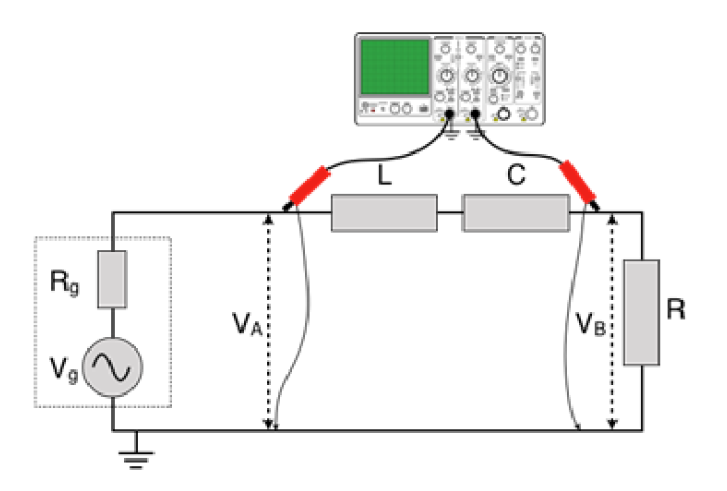
\includegraphics{configRLC.png}}
    \caption{Configurazione circuito RLC}
    \label{fig:configRLC}
\end{figure}

\subsection{Dati raccolti RLC} 
Di seguito riportiamo i dati raccolti per il circuito RLC. Dopo aver riprodotto lo stesso circuito rappresentato nella figura \ref{fig:configRLC} abbiamo posizionato le sonde dell'oscilloscopio: sonda 1 per misurare $V_\text{in}$ ai capi del generatore e sonda 2 per misurare $V_\text{out}$ ai capi della resistenza. A causa dei problemi con i dati riscontrati nella prima sezione e la conseguente perdita di tempo abbiamo deciso di valutare la funzione di trasferimento per L e C unite, invece che per L e C separatamente. Le componenti utilizzate per questo circuito sono:
\begin{enumerate}
	\item Resistenza $(R = 1000\pm0.1) \Omega$
        \item Capacità $C = 10\ \text{nF} $
	\item Induttore $L = (0.05\pm0.01) \text{H}$
\end{enumerate}
Successivamente abbiamo misurato i seguenti parametri al variare della frequenza imposta dal generatore, in un range tra 1 kHz e 150 kHz:
\begin{enumerate}
	\item Ampiezza del segnale $V_\text{in}$
	\item Ampiezza del segnale $V_\text{out}$
	\item Ampiezza della differenza $V_\text{in} - V_\text{out}$
	\item Differenza di fase tra $V_\text{in} - V_\text{out}$ e $V_\text{in}$
	\item Differenza di fase tra $V_\text{in}$ e $V_\text{out}$
\end{enumerate}

\subsection{Analisi Dati RLC}

\subsubsection{Ai capi della resistenza}
Dopo aver raccolto i dati in modo analogo a quanto fatto per i circuiti RC ed RL, abbiamo calcolato il modulo e la fase della funzione di trasferimento ai capi della resistenza.\\
Di seguito vengono riportati i dati per il modulo della funzione di trasferimento, con relativa interpolazione eseguita con la forma funzionale \ref{eq:Modulo RLC (resistenza)}.  

%Figure da inserire: grafico interpolazione e
\begin{figure}[h!]
    \centering
    \resizebox{0.7\textwidth}{!}{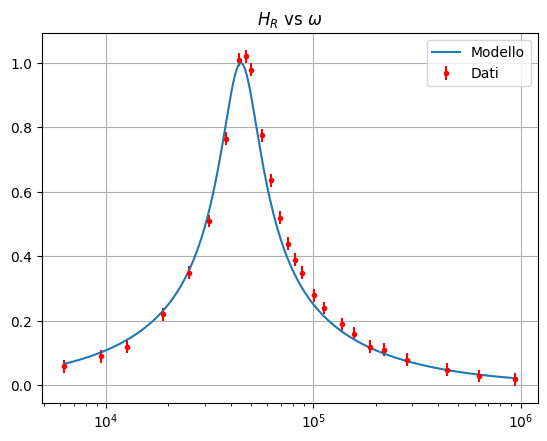
\includegraphics{RLC_R_modulo.png}}
    \caption{Modulo funzione Trasferimento per resistenza in RLC}
    \label{fig:RLC_R_modulo}
\end{figure}
I valori ottenuti dal fit sono:
\begin{enumerate}
    \item Resistenza  $R = (1088\pm165) \Omega $
    \item Induttanza  $L = (0.047\pm0.007) \text{H} $
    \item Capacità    $C = (9.7\pm1.5) \text{nF} $
\end{enumerate}
La concordanza del modello è stata valutata tramite il test del $\chi^2$; di seguito riportiamo i risultati ottenuti.

Concordanza del modello per il modulo:
\begin{enumerate} 
    \item: $\widetilde{\chi}^2 = 0.4$   
    \item: $p-value = 0.99$ 
\end{enumerate}

Abbiamo interpolato i dati della fase tramite la forma funzionale \ref{eq:Fase RLC (resistenza)}.

%Figure da inserire: grafico interpolazione e
\begin{figure}[h!]
    \centering
     \resizebox{0.7\textwidth}{!}{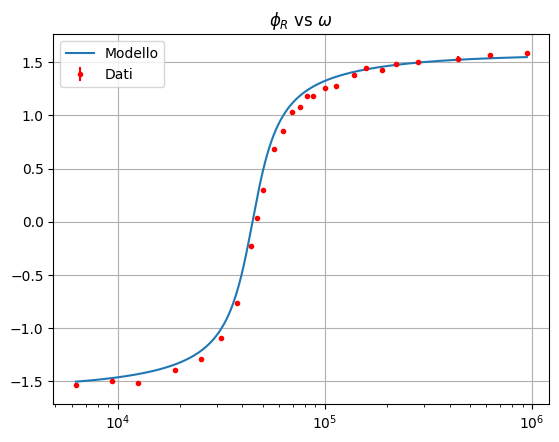
\includegraphics{RLC_R_fase.png}}
    \caption{Grafico fase funzione di Trasferimento per resistenza in RLC}
    \label{fig:RLC_R_fase}
\end{figure}

I valori ottenuti dal fit sono:
\begin{enumerate}
    \item Resistenza  $R = (1060\pm %non so cosa mettere qui come incertezza%
    )\ \Omega $
    \item Induttanza  $L = (0.047\pm)\ \text{H} $
    \item Capacità    $C = (9.52\pm)\ \text{nF} $
\end{enumerate}
La concordanza del modello è stata valutata tramite il test del $\chi^2$; di seguito riportiamo i risultati ottenuti.
R = 1.06e+03 pm 2.62e+03
L = 0.0477 pm 0.118
C = 9.51e-09 pm 2.36e-08
Concordanza del modello per la fase:
\begin{enumerate} 
    \item: $\widetilde{\chi}^2 = 1.3$   
    \item: $p-value = 0.16$ 
\end{enumerate}

\subsubsection{Ai capi di LC}
A causa dello scarso tempo rimanente, siamo riusciti a prendere le misurazioni della tensione solamente ai capi del sistema induttanza-capacità, e non dei due componenti singolarmente; pertanto la nostra analisi osserverà solamente le funzioni di trasferimento attorno a LC. \\
Di seguito riportiamo i dati per il modulo e la fase della funzione di trasferimento ai capi di LC con relativa interpolazione. Le forme funzionali utilizzate per il fit seguono le relazioni: \eqref{eq:Modulo RLC (capacita)}  per il modulo, e \eqref{eq:Fase RLC (capacita)} per la fase.

\begin{figure}[h!]
    \centering
    \resizebox{0.7\textwidth}{!}{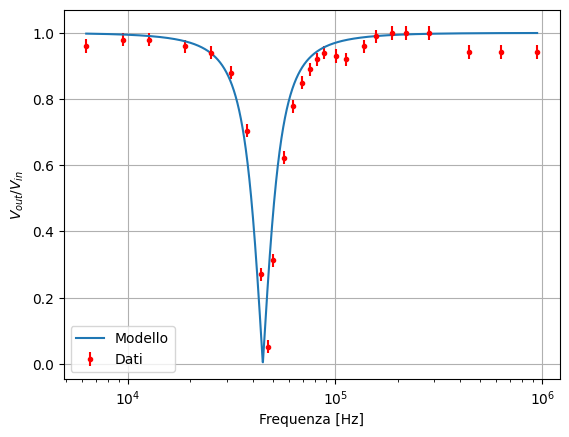
\includegraphics{RLC_L_modulo.png}}
    \caption{Grafico modulo funzione di Trasferimento per sistema induttanza-capacità in RLC}
    \label{fig:RLC_LC_modulo}
\end{figure}

\paragraph{Fit del modulo della funzione di trasferimento}
I valori di R, L e C estratti dal fit dei dati sono i seguenti:

\begin{enumerate}
    \item Resistenza $R = (1050 \pm 90)\ \Omega$
    \item Induttanza $L = (0.048 \pm 0.004)\ $ H
    \item Capacità $C = (9.5 \pm 0.8)\ $ nF
\end{enumerate}

\begin{figure}[h!]
    \centering
    \resizebox{0.7\textwidth}{!}{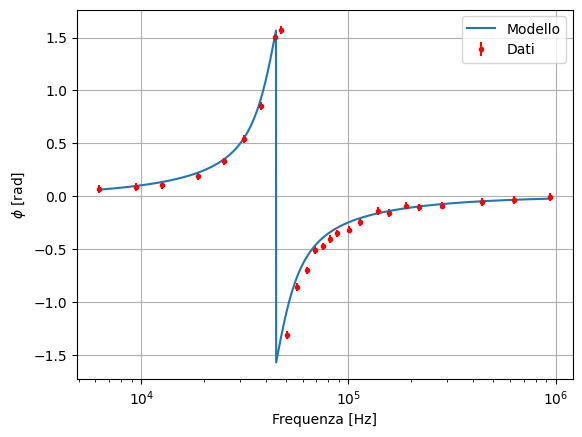
\includegraphics{RLC_L_fase.png}}
    \caption{Grafico fase funzione di Trasferimento per sistema induttanza-capacità in RLC}
    \label{fig:RLC_LC_fase}
\end{figure}

Effettuando un test di compatibilità tra le misure effettuate ed il modello si ottengono i seguenti risultati:

\begin{enumerate} 
    \item: $\widetilde{\chi}^2 = 2.0$   
    \item: $p-value = 0.002$ 
\end{enumerate}

Eseguendo infine un t-test tra i valori dei parametri misurati e quelli estratti dal fit, si ottiene una distanza in deviazioni standard dal valore atteso di:

\begin{enumerate}
    \item R \quad  $t = 0.86$
    \item L \quad $t = 0.95$
    \item C \quad $t = 0.97$
\end{enumerate}

\paragraph{Fit della fase della funzione di trasferimento}
Per quanto riguarda la fase, dal grafico \ref{fig:RLC_LC_fase} si osserva chiaramente una discontinuità nella differenza di fase misurata. La libreria utilizzata per eseguire il fit (Minuit) non è adatta ad operare con dati del genere. \\ %non mi piace troppo sto termine
Per questo motivo abbiamo separato il set di misure in due, in modo da fittare separatamente le due parti della curva, e ottenuto due stime distinte per i parametri. Successivamente, per ricavare la miglior stima dei parametri, abbiamo combinato i valori secondo una media aritmetica e le incertezza sotto media in quadratura.

\begin{enumerate}
    \item $R_1 = (913 \pm 159)\ \Omega \,, \quad R_2 = (1070 \pm 1170)\ \Omega \implies R_{best} = (992 \pm 1180)\ \Omega$
    
    \item $L_1 = (0.050 \pm 0.008)\ \text{H} \,, \quad L_2 = (0.048 \pm 0.053)\ \text{H} \implies L_{best} = (0.049 \pm 0.053)\ \text{H}$

    \item $C_1 = (9.98 \pm 1.65)\ \text{nC} \,, \quad C_2 = (9.4 \pm 10.2)\ \text{nC} \implies C_{best} = (9.7 \pm 10.4)\ \text{nC}$

\end{enumerate}

Abbiamo sottoposto entrambi i fit ad un test di compatibilità, ottenendo nel primo caso:

$$ \widetilde{\chi}^2 = 0.3, \quad p-value = 0.92 $$

mentre nel secondo caso:

$$ \widetilde{\chi}^2 = 2.3, \quad p-value = 0.003 $$


\subsection{Conclusioni sul circuito RLC}

\subsubsection{Funzioni di trasferimento sulla resistenza}
Per quanto riguarda le misure fatte sulla resistenza, dai test di compatibilità effettuati possiamo confermare la compatibilità delle misure con il modello per le funzioni di trasferimento attese. \\ 
La "bell curve" risultante dal grafico del modulo\ref{fig:RLC_R_modulo} rappresenta la risposta della resistenza e in generale di tutto il circuito. La \textbf{larghezza} della campana è legata al range di frequenze imposte sul circuito e rispecchia l'intervallo in cui il circuito risponde in modo significativo, una maggiore R corrisponde ad una campana più larga e dunque un intervallo di frequenze maggiore.
\textbf{L'altezza} della campana invece è legata alla "forza" della risposta del circuito, se sono presenti risonanze i valori si sommano e il picco si alzerà.
Possiamo inoltre trarre delle conclusioni per la risposta in frequenza del circuito per certi valori di R che come sappiamo determinano il \textbf{regime} di tale circuito: sottosmorzato, sovrasmorzato e criticamente smorzato.
Tenendo conto di che cosa ci si aspetta da ciascuno dei tre casi, guardando il grafico da noi ottenuto è possibile riconoscere un sistema sottosmorzato, questo perché la presenza di un picco ad una determinata frequenza indica un fenomeno di risonanza, inoltre come ci si aspetta dopo tale frequenza di risonanza, l'ampiezza della risposta segue un graduale decadimento senza incontrare nuovi picchi, mimando lo smorzamento che appunto rallenta l'oscillazione del circuito. Per altri regimi, ad esempio quello sovrasmorzato, ci si aspetterebbe invece l'assenza di fenomeni di risonanza, ciò è dovuto al fatto che un sovrasmorzato oppone molta resistenza all'oscillazione. Dunque ogni regime riflette le proprie caratteristiche nella risposta in frequenza.\\

\subsubsection{Funzioni di trasferimento su induttanza e capacità}
Per quanto riguarda la seconda parte relativa al fit del modulo della funzione di trasferimento su LC, il test di compatibilità tra misure ci conferma la bontà della stima dei parametri. Il $\widetilde\chi^2$ di 2 e un p-value basso, ci suggeriscono una leggera discrepanza tra il modello e i dati raccolti. \\
Questo può essere dovuto a molti fattori, come all'aver preso le misure a frequenze piu' alte in un secondo momento, o all'aver sottostimato gli errori presenti.

\\
Infine, studiando la fase di $H(\omega)$ di LC, ci accorgiamo che si ripresentano alcuni dei problemi osservati in precedenza. In particolare il fatto che l'incertezza sulle misure estratte dal fit sia maggiore del valore stesso del parametro, nonostante un valore di $\widetilde\chi^2$ non particolarmente alto. Abbiamo tentato di spiegare questo fatto in diversi modi.\\
Una probabile spiegazione è la scarsa qualita dei dati raccolti, giustificabile almeno in parte dai numerosi problemi tecnici accaduti durante l'esperienza. Un'altra possibile motivazione è il fatto che i nostri dati non seguano a pieno il modello previsto, dal momento che diversi fattori possono influire su questo aspetto, come la presenza di induttanze/capacità non previste, una configurazione del circuito non ottimale o possibili comportamenti non lineari dei componenti, come già osservato nel punto \ref{subsec:Modulo RC}.

\subsection{Inciso sulle incertezze} \label{sec:incertezze}
Nello svolgimento dell'analisi dati, abbiamo tenuto conto degli errori sulle misure basandoci sulla precisione dell'oscilloscopio.\\
Al fine di leggere chiaramente i valori rilevati dallo strumento, abbiamo impostato una media su 64 cicli e osservato l'ampiezza massima delle oscillazioni nel valore riportato. Dopo la prima decina di misure, ci siamo resi conto del fatto che la lettura oscillava tra circa $\pm\, 20$ mV dal valore medio, dunque abbiamo preso questo come valore standard per le nostre incertezze.\\
Per ottenere l'errore su $H(\omega) = \frac{V_{out}}{V_{in}}$, abbiamo propagato l'errore tramite la formula:

$$\sigma_H = \sqrt{\left(\frac{\sigma_{out}}{V_{in}}\right)^2 + \left(\frac{V_{out}}{V_{in}}\right)^2 \cdot \sigma_{in}^2}$$

Infine, per stimare l'errore sullo sfasamento tra i segnali, abbiamo ripetuto la stessa procedura fatta per quello sul modulo. Questa volta però, la lettura del valore è risultata più stabile consentendoci di stabilire con sicurezza un errore di 1 grado, convertito poi in radianti. \\

\paragraph{Valori di incertezza elevati} In diversi dei nostri risultati, riscontriamo un'incertezza di molto superiore al valore stesso del parametro stimato tramite fit.
Eseguendo una stima a posteriori dell'incertezza da assegnare alle misure, abbiamo notato che dopo un leggero aumento dell'errore, il $\widetilde\chi^2$ tendeva a 1, ma l'imprecisione sulla stima dei parametri del modello aumentavano rapidamente. Per questo motivo abbiamo deciso di tenere l'incertezza valutata inizialmente e continuare con l'analisi.

\newpage
\section{Tabelle misurazioni}
\begin{table}[htbp]
    \centering
    \caption{Dati RC}
    \resizebox{0.8\textwidth}{!}{
    \begin{tabular}{ccccccc}
        \toprule
        Frequenza & Ampiezza Va & Ampiezza Vb & Ampiezza Va-b & ddf a/b & ddf a-b/a \\
        \midrule
        200 & 10.2 & 0.17 & 10.17 & 92.0 & 0.6 \\
        400 & 10.19 & 0.25 & 10.2 & 90.5 & 1.2 \\
        600 & 10.19 & 0.37 & 10.21 & 89.8 & 2.0 \\
        800 & 10.17 & 0.49 & 10.22 & 89.3 & 2.7 \\
        1000 & 10.18 & 0.62 & 10.23 & 87.5 & 3.4 \\
        2000 & 10.0 & 1.28 & 10.06 & 85.3 & 4.1 \\
        3000 & 9.9 & 1.92 & 9.9 & 82.2 & 8.6 \\
        4000 & 9.8 & 2.55 & 9.7 & 78.4 & 14.5 \\
        5000 & 9.66 & 3.1 & 9.4 & 75.5 & 18.2 \\
        6000 & 9.45 & 3.6 & 9.1 & 73.0 & 21.7 \\
        8000 & 9.08 & 4.46 & 8.3 & 65.1 & 25.9 \\
        10000 & 8.74 & 5.13 & 7.67 & 59.5 & 35.3 \\
        12000 & 8.45 & 5.58 & 7.05 & 54.3 & 40.6 \\
        13000 & 8.36 & 5.82 & 6.75 & 52.8 & 40.7 \\
        14000 & 8.23 & 5.98 & 6.46 & 50.7 & 44.5 \\
        15000 & 8.1 & 6.15 & 6.25 & 48.2 & 48.9 \\
        15500 & 8.075 & 6.18 & 6.06 & 47.9 & 50.1 \\
        16000 & 8.05 & 6.28 & 5.95 & 46.0 & 50.4 \\
        16500 & 7.9 & 6.32 & 5.88 & 46.2 & 51.8 \\
        17000 & 7.9 & 6.38 & 5.74 & 45.5 & 49.5 \\
        18000 & 7.8 & 6.48 & 5.54 & 43.1 & 54.1 \\
        19000 & 7.77 & 6.6 & 5.31 & 42.2 & 54.5 \\
        20000 & 7.75 & 6.65 & 5.13 & 40.7 & 58.4 \\
        22000 & 7.6 & 6.8 & 4.77 & 37.8 & 62.5 \\
        30000 & 7.29 & 7.14 & 3.72 & 26.6 & 73.5 \\
        40000 & 7.13 & 7.39 & 2.9 & 22.1 & 83.9 \\
        50000 & 7.05 & 7.45 & 2.4 & 17.9 & 90.2 \\
        100000 & 6.94 & 7.52 & 1.39 & 8.8 & 112.0 \\
        150000 & 6.9 & 7.56 & 1.08 & 7.2 & 125.0 \\
        300000 & 6.91 & 7.6 & 0.84 & 4.5 & 144.0 \\
        500000 & 6.91 & 7.63 & 0.83 & 1.4 & 162.0 \\
        1000000 & 6.9 & 7.6 & 0.78 & 1.1 & 170.0 \\
        1500000 & 6.94 & 7.63 & 0.77 & 0.9 & 171.0 \\
        3000000 & 6.96 & 7.6 & 0.74 & 0.0 & 178.0 \\
        \bottomrule
    \end{tabular}}
\end{table}
\begin{table}[htbp]
    \centering
    \caption{Dati RL}
    \begin{tabular}{cccccc}
        \toprule
        Frequenza & Ampiezza Va & Ampiezza Vb & Ampiezza Va-b & ddf a/b & ddf a-b/a \\
        \midrule
        100 & 10.0 & 9.8 & 0.4 & 0 & -84.0 \\
        250 & 9.9 & 9.8 & 0.7 & 1 & -80.0 \\
        400 & 9.9 & 9.8 & 0.7 & 1 & -75.0 \\
        500 & 9.6 & 9.04 & 1.36 & 7 & -68.0 \\
        700 & 9.6 & 9.04 & 1.84 & 10 & -69.0 \\
        900 & 9.6 & 8.9 & 2.2 & 12 & -63.0 \\
        1100 & 9.6 & 8.8 & 2.64 & 15 & -62.0 \\
        1400 & 9.6 & 8.7 & 3.04 & 19 & -66.0 \\
        1700 & 9.7 & 8.4 & 3.6 & 23 & -62.0 \\
        2000 & 9.76 & 8.32 & 4.24 & 26 & -60.0 \\
        2200 & 9.76 & 8.1 & 4.56 & 29 & -58.0 \\
        2400 & 9.76 & 8.0 & 4.88 & 31 & -56.0 \\
        2600 & 9.76 & 7.76 & 5.2 & 33 & -51.0 \\
        2700 & 9.76 & 7.68 & 5.36 & 35 & -51.0 \\
        2800 & 9.76 & 7.68 & 5.52 & 35 & -50.0 \\
        2900 & 9.76 & 7.5 & 5.68 & 37 & -49.0 \\
        3000 & 9.76 & 7.44 & 5.84 & 36 & -48.0 \\
        3100 & 9.76 & 7.36 & 5.92 & 38 & -47.0 \\
        3200 & 9.76 & 7.28 & 6.0 & 39 & -47.0 \\
        3300 & 9.76 & 7.2 & 6.16 & 40 & -46.0 \\
        3400 & 9.76 & 7.12 & 6.3 & 41 & -46.0 \\
        3500 & 9.76 & 7.04 & 6.4 & 41 & -45.0 \\
        3700 & 9.76 & 6.88 & 6.64 & 43 & -45.0 \\
        4000 & 9.84 & 6.64 & 6.88 & 45 & -42.0 \\
        4500 & 9.92 & 6.24 & 7.28 & 49 & -38.0 \\
        5000 & 9.92 & 5.84 & 7.68 & 52 & -36.0 \\
        6000 & 9.92 & 5.2 & 8.16 & 58 & -31.0 \\
        7000 & 10.0 & 4.64 & 8.56 & 60 & -28.0 \\
        8000 & 10.0 & 4.24 & 8.8 & 64 & -25.0 \\
        10000 & 10.0 & 3.6 & 9.12 & 68 & -20.0 \\
        15000 & 10.08 & 2.48 & 9.6 & 76 & -14.0 \\
        20000 & 10.08 & 1.8 & 9.4 & 79 & -9.0 \\
        30000 & 10.2 & 1.28 & 9.6 & 83 & -9.0 \\
        50000 & 10.4 & 0.8 & 9.6 & 85 & -6.0 \\
        75000 & 10.4 & 0.48 & 9.8 & 89 & -2.0 \\
        100000 & 10.4 & 0.34 & 9.8 & 89 & -0.5 \\
        \bottomrule
    \end{tabular}
\end{table}

\begin{table}[htbp]
    \centering
    \caption{Dati RLC}
    \begin{tabular}{cccccc}
        \toprule
        Frequenza & Ampiezza Va & Ampiezza Vb & Ampiezza Va-b & ddf a/b & ddf a-b/a \\
        \midrule
        1000 & 10.2 & 0.6 & 9.8 & -88 & 4.0 \\
        1500 & 10.0 & 0.9 & 9.8 & -86 & 5.0 \\
        2000 & 10.0 & 1.2 & 9.8 & -87 & 6.0 \\
        3000 & 10.0 & 2.2 & 9.6 & -80 & 11.0 \\
        4000 & 10.0 & 3.5 & 9.4 & -74 & 19.0 \\
        5000 & 10.0 & 5.1 & 8.8 & -63 & 31.0 \\
        6000 & 9.8 & 7.5 & 6.9 & -44 & 49.0 \\
        7000 & 9.6 & 9.7 & 2.6 & -13 & 86.0 \\
        7500 & 9.6 & 9.8 & 0.5 & 2 & 90.0 \\
        8000 & 9.6 & 9.4 & 3.0 & 17 & -75.0 \\
        9000 & 9.8 & 7.6 & 6.1 & 39 & -49.0 \\
        10000 & 9.9 & 6.3 & 7.7 & 49 & -40.0 \\
        11000 & 10.0 & 5.2 & 8.5 & 59 & -29.0 \\
        12000 & 10.0 & 4.4 & 8.9 & 62 & -27.0 \\
        13000 & 10.0 & 3.9 & 9.2 & 68 & -23.0 \\
        14000 & 10.0 & 3.5 & 9.4 & 68 & -20.0 \\
        16000 & 10.0 & 2.8 & 9.3 & 72 & -18.0 \\
        18000 & 10.0 & 2.4 & 9.2 & 73 & -14.0 \\
        22000 & 10.0 & 1.9 & 9.6 & 79 & -8.0 \\
        25000 & 10.0 & 1.6 & 9.9 & 83 & -9.0 \\
        30000 & 10.0 & 1.2 & 10.0 & 82 & -5.0 \\
        35000 & 10.0 & 1.1 & 10.0 & 85 & -6.0 \\
        45000 & 10.0 & 0.8 & 10.0 & 86 & -5.0 \\
        70000 & 10.4 & 0.5 & 9.8 & 88 & -3.0 \\
        100000 & 10.4 & 0.3 & 9.8 & 90 & -2.0 \\
        150000 & 10.4 & 0.19 & 9.8 & 91 & -0.4 \\
        \bottomrule
    \end{tabular}
\end{table}


\end{document}
